
\chapter{Non-local Methods}
In the following sections, we introduce non-local methods
to create curves from data points.  Thereafter, we
introduce local methods.
Non-local methods mean that any change in a data point (or a control point) 
affects 
the {\em entire} curve.  This is generally undesirable.  
However, non-local methods are simpler than local methods, so they 
are introduced first.  Table~\ref{tab:concept_map} presents an overview
of the four methods to be covered, categorized by interpolation and 
locality.

\begin{table}[htb]
\caption{Categorization of methods by interpolation and locality.}
% \centering
\begin{center}
\begin{tabular}{cc||c|c}
& & \multicolumn{2}{c}{\bf Locality} \\
& & non-local methods & local methods \\
& & ``curves'' & ``splines'' \\
\hline \hline
\multirow{2}{*}{\bf Interpolation} & data points & polynomial & spline \\ \cline{2-4}
& control points & B\'ezier, Bernstein & B-spline, NURB \\
\end{tabular}
\end{center}
\label{tab:concept_map}
\end{table}
In general, we will refer to non-local methods as {\bf curves} of 
degree $p$, denoted
$f_p(x) \in \real$ for non-parameterized curves (univariate polynomials, as
in Table~\ref{tab:polynomials}) and 
$\vC_p(t; \vx) \in \realthree$ for parameterized curves (B\'ezier curves written
in the Bernstein basis, as in (\ref{eq:general_bezier_curve})).  
In contrast, we will refer to local methods as {\bf splines} of 
degree $p$, denoted $S_p(t; x) \in \real$ and 
$\vS_p(t; \vx) \in \realthree$ (used throughout Chapter~\ref{chapter:local_methods}).

\section{Polynomials}
We briefly discuss polynomials for three main reasons:  
(1)~To be explicit
regarding the terminology of {\bf power} versus {\bf order} and be clear
on the conventions and notations used in this document, 
(2)~to lay the framework
for more sophisticated interpolations that will rely on polynomials in some 
form, and 
(3)~to
the  note shortcomings of polynomials and thus motivate alternative 
approaches.

First, with regard to {\em power} versus {\em order}, \cite{Cottrell-2009}
noted the following:

\begin{Hquote}
Page 18, Note 3: ``There is a terminology conflict between the geometry and analysis communities. 
Geometers will say a cubic polynomial has degree 3 and order 4.  In geometry,
order equals degree plus one.  Analysts will say a cubic polynomial is order
three, and use the term order and degree synonymously.  This is the convention
we [Cottrell, Hughes, Bazilevs] adhere to.'' 
\end{Hquote}

Unlike \cite{Cottrell-2009}, we adopt the geometry community 
convention in this document, thus 
we distinguish between {\em order} and {\em power}.  
We have elected this approach primarily for consistency of this 
document with historical writings of the geometry community.

Next, there is some basic notation used with polynomials that we need 
to make clear and concrete.  
Let $f_p(x)$ be the function of degree $p$ 
(equivalently, order $p+1$) that is a sum of variable
$x$ raised to some increasing non-negative integer power, starting 
from zero, and multiplied
by a constant coefficient $a$, such that
\be
f_p(x) \defe
a_0 x^0 + a_1 x^1 + a_2 x^2 + a_3 x^3 + \cdots + a_p x^p = 
\sum_{i=0}^p a_i x^i.
\ee
The function $f_p(x)$ is a {\bf polynomial} of {\bf degree} $p$, the highest
non-zero {\bf power}\footnote{We suggest the mnemonic of ``$p$'' as the 
index used for the ``\underline{p}ower'' in a ``\underline{p}olynomial.''} used in the summation.  
Table~\ref{tab:polynomials} lists
the first five polynomials by order, degree, name, and function.  
Hereinafter, $p$ will be considered the index of the 
power of a polynomial.  The $p$-index, a subset of non-negative integers, 
will start from zero and consecutively increase by one.

\begin{table}[htb]
\caption{First five orders of a polynomial function.}
% \centering
\begin{center}
\begin{tabular}{c|c|l|l}
{\bf order} & {\bf degree} & {\bf name} & {\bf function} \\
\hline \hline
$\mathcal{O}(1)$ & $p=0$ & constant & $f_0(x) = a_0$ \\
$\mathcal{O}(2)$ &  $p=1$ & linear & $f_1(x) = a_0 + a_1 x$ \\
$\mathcal{O}(3)$ & $p=2$ & quadratic & $f_2(x) = a_0 + a_1 x + a_2 x^2$ \\
$\mathcal{O}(4)$ & $p=3$ & cubic & $f_3(x) = a_0 + a_1 x + a_2 x^2 + a_3 x^3$ \\
$\mathcal{O}(5)$ & $p=4$ & quartic & $f_4(x) = a_0 + a_1 x + a_2 x^2 + a_3 x^3 + a_4 x^4$ \\
\end{tabular}
\end{center}
\label{tab:polynomials}
\end{table}

One note regarding conventions of indices.  We use the first
item of a series {\tt s} to be {\tt s[0]}, the second item to be 
{\tt s[1]}, and so forth.  We prefer the zero-based indices because 
it is consistent not only with our work in Python, which is zero-based, 
but also with concepts from initial boundary value problems (IBVPs), 
which denote initial conditions, the first values, as occurring at $t_0$.

Finally, we state as {\em prima facie} a well-known shortcoming of polynomials
is their propensity to overfit the data.  This characteristic arises because
a polynomial of degree $p$ has $p-1$ changes of direction, from $-f_p(x)$ to
$f_p(x)$, or vice versa.  No further discussion on overfitting is given here, 
though explications of this topic are widely available.  


\section{B\'ezier Curves}
\label{sec:bezier_curves}
Several of the ideas in this section are due to the excellent references
of \cite{Bartels-1995}, \cite{Piegl-2012}, \cite{Rogers-2000}, 
and \cite{Shiach-2015}.
A B\'ezier curve is a parametric curve defined by control points.
A control point $\vP_i$ will have two coordinates $(x_i, y_i)$ in 2D and
three coordinates $(x_i, y_i, z_i)$ in 3D.
The parameter is typically denoted $t$.  The bounds for $t$ are 
$0 \leq t \leq 1$ unless otherwise indicated.

Here, $t$ does not denote time, as is customary in solid mechanics.  
Rather, $t$ can be thought of as a ``pseudo-time,'' wherein the 
parameterization flows from beginning to end of the $t$ bounds.
Also, the bounds of $t$ will later be shown to be arbitrary.  For now, 
however, it is much more convenient to state the bounds as between zero
and one.

A B\'ezier curve of degree $p$ requires $p+1$
control points. For example, a B\'ezier 
curve that is a line (degree $p=1$) requires two control points.
Affine transformations may be used to modify the control points, \eg to 
scale, reflect, rotate, or translate (offset) the control points.

\subsection{B\'ezier Line}
Let $\vP(t; \vx) \in \realthree$ be {\bf parametric} equation for a line between 
two points $\vP_0 = (x_0, y_0, z_0)$ and $\vP_1 = (x_1, y_1, z_1)$, with
$\vx = (x, y, z)$.
Then, let $t$ be the parameter bounded by $0 \leq t \leq 1$.  Then 
the B\'ezier line between $\vx_0$ and $\vx_1$ is simply the parameterized 
linear interpolation $\vP_0$ and $\vP_1$, 
\be
\vP(t; \vP_0, \vP_1) \defe (1 - t) \vP_0 + t \vP_1, 
\ee
or in explicit coordinate form,
\be
\left\{\begin{tabular}{c} $x(t)$ \\ $y(t)$ \\ $z(t)$ \end{tabular} \right\}
= 
(1 - t)
\left\{\begin{tabular}{c} $x_0$ \\ $y_0$ \\ $z_0$ \end{tabular} \right\}
+ 
t \left\{\begin{tabular}{c} $x_1$ \\ $y_1$ \\ $z_1$ \end{tabular} \right\}.
\ee

\subsection{B\'ezier Quadratic}
Let $\vQ(t; \vx)$ be the parametric equation for a quadratic between two points
$\vQ_0$ and $\vQ_1$.  Let the position of these two points themselves be 
parameterized by three points $\vP_0$, $\vP_1$, and $\vP_2$, such that
\begin{align}
\vQ_0(t; \vP_0, \vP_1) & = (1 - t) \vP_0 + t \vP_1,
\label{eq:bezier_quad_one}
\\
\vQ_1(t; \vP_1, \vP_2) & = (1 - t) \vP_1 + t \vP_2.
\label{eq:bezier_quad_two}
\end{align}
Thus, the position of $\vQ_0$ is on the line between points $\vP_0$ and 
$\vP_1$.  The position of $\vQ_1$ is on the line between points $\vP_1$ and 
$\vP_2$.
At $t=0$, $\vQ_0$ resides at $\vP_0$, $\vQ_1$ resides at $\vP_1$.  
At $t=1$, $\vQ_0$ resides at $\vP_1$, $\vQ_1$ resides at $\vP_2$.
Finally, let position along the quadratic B\'ezier curve $\vQ(t; \vx)$ 
be defined as 
\be
\vQ(t; \vQ_0, \vQ_1) \defe (1 - t) \vQ_0 + t \vQ_1.
\ee
This curve can be recast in terms of the three points $\vP_0$, $\vP_1$, 
and $\vP_2$ by substituting
(\ref{eq:bezier_quad_one}) and
(\ref{eq:bezier_quad_two}),
\be
\vQ(t; \vP_0, \vP_1, \vP_2) = (1-t)^2 \vP_0 + 2t (1-t) \vP_1 + t^2 \vP_2.
\label{eq:bezier_quadratic}
\ee
Figure~\ref{fig:de_casteljau}(a) illustrates 
an example quadratic B\'ezier curve, with the three control 
points $\vP_0$, $\vP_1$, and $\vP_2$ indicated.\footnote{We do
not call $\vQ_0$ and $\vQ_1$ control points, since they are dependent
on $\vP_0$, $\vP_1$, and $\vP_1$ through parameter $t$ in 
(\ref{eq:bezier_quad_one}) 
and (\ref{eq:bezier_quad_two}).}$^,$\footnote{Figure~\ref{fig:de_casteljau}(b)
shows the same curve as in Figure~\ref{fig:de_casteljau}(a), just with 
a recursive notation, discussed in Section~\ref{sec:de_casteljau}.}
We will designate the number of control points to be $(n+1)$.  
Thus, the number of control points in the 
current example (Figure~\ref{fig:de_casteljau})
is $(n+1) = 3 \implies n=2$.  Each control
point can be identified in sequence as $\vP_i$, with $i = 0, 1, \ldots n$.
The maximum 
degree B\'ezier that can be constructed is two 
(degree $p$ requires $p+1$ control points).  Thus we see 
for a series of $(n+1)$ control points, we can construct a 
B\'ezier curve of degree $p=n$.

\begin{figure}[htb]
  \begin{center}
    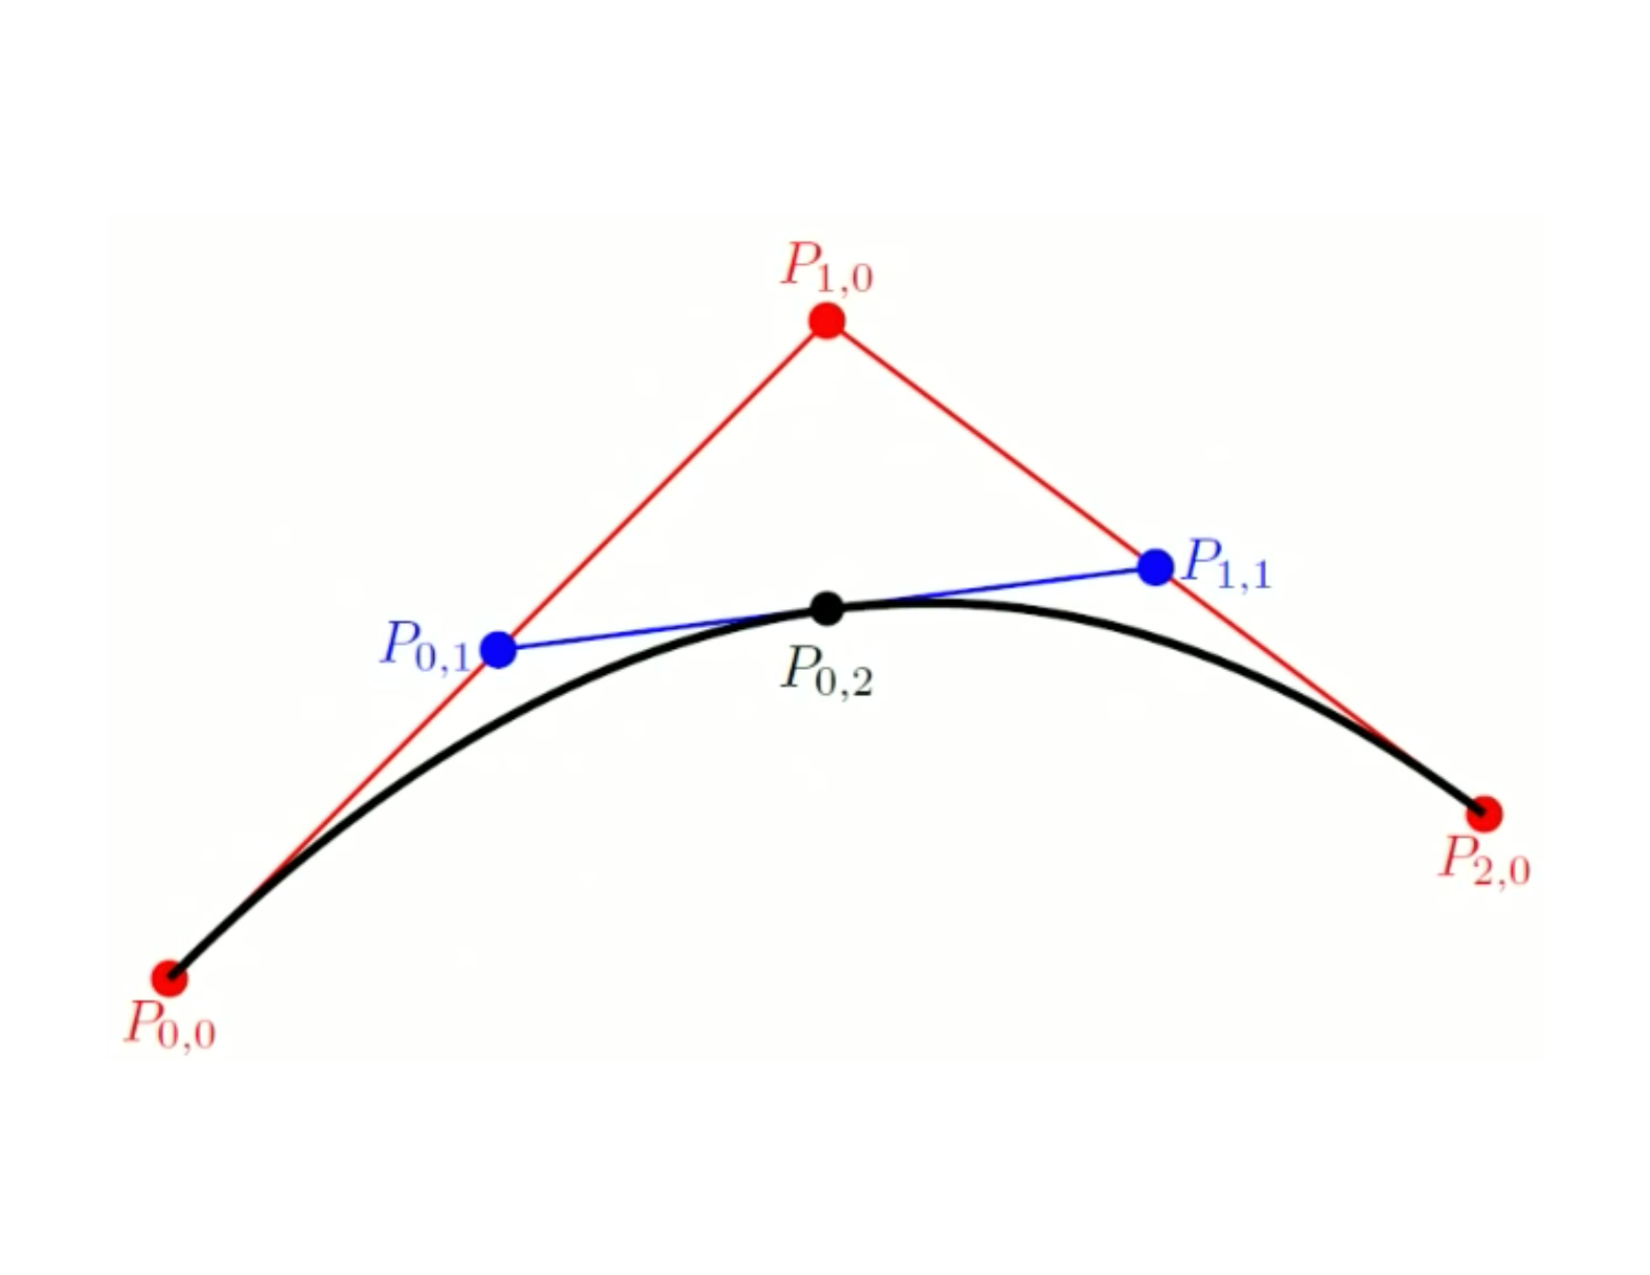
\includegraphics[width=\textwidth]{fig/de_casteljau.pdf}
  \end{center}
    \caption{A B\'ezier quadratic curve illustrated at $t=0.5$
    with (a) original notation 
    and (b) the de Casteljau's algorithm notation.  
    Reference: fig/de\_casteljau.py.}
  \label{fig:de_casteljau} % label must come after caption 
\end{figure}

\begin{Hexpo}
{Figure~\ref{fig:de_casteljau_sequence} illustrates the same quadratic
B\'ezier curve shown in Figure~\ref{fig:de_casteljau}, generated at  
six discrete points in the interval $t \in [0, 1]$.
\begin{figure}[htb]
  \begin{center}
    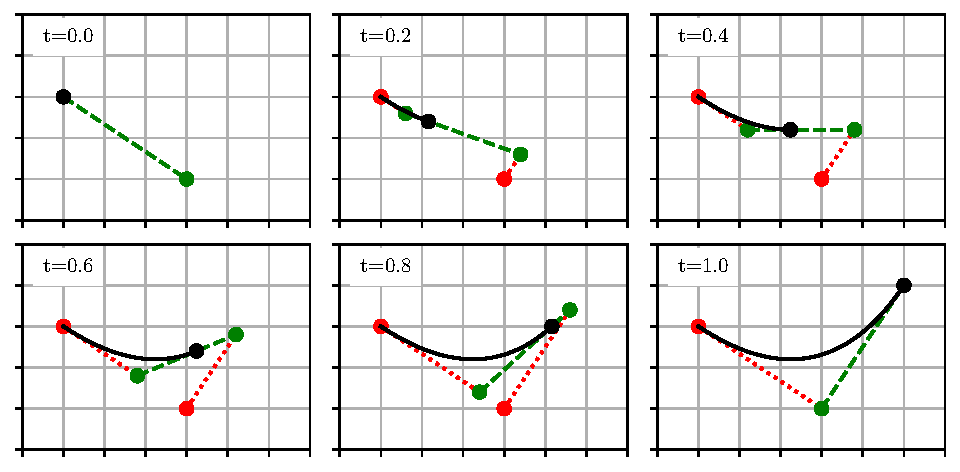
\includegraphics[width=\textwidth]{fig/de_casteljau_sequence.pdf}
  \end{center}
    \caption{The B\'ezier quadratic curve discussed in 
    Figure~\ref{fig:de_casteljau}, 
    illustrated in sequence with $t$ starting at 0 and ending at 1.
    Reference: fig/de\_casteljau.py.}
  \label{fig:de_casteljau_sequence} % label must come after caption 
\end{figure}
}
\end{Hexpo}

With these Figures~\ref{fig:de_casteljau}--\ref{fig:de_casteljau_sequence} 
in mind, a few additional observations\footnote{These items
are stated as true but not proven here. Consult
the references in the Bibliography section for proofs.} can be made:
\begin{itemize}
 \item The control points sequence $\vP_0$, $\vP_1$, $\vP_2$ is a coarse 
 and discrete {\em approximation} the continuous quadratic B\'ezier curve
 $\vQ(t)$.
 \item The end points, $\vP_0$ and $\vP_2$, are interpolated, but 
 the interior point $\vP_1$ is not
 interpolated.\footnote{This will generalize to all interior points for
 higher-degree B\'ezier curves.}
 \item The tangent of the curve $\vQ(t)$ at $t=0$ is parallel to the line
 $\vP_1 - \vP_0$.
 The tangent of the curve $\vQ(t)$ at $t=1$ is parallel to the line
 $\vP_2 - \vP_0$.
 \item The entire curve $\vQ(t)$ is contained in the triangle formed with vertices
 $\vP_0$, $\vP_1$, $\vP_2$.
\end{itemize}




\newpage
\subsection{de Casteljau's Algorithm}
\label{sec:de_casteljau}
The foregoing development can be generalized, and is known as 
{\bf de Casteljau's algorithm}.  Let $\vP_{i,j}$ be control points
where 
\begin{itemize}
\item $i$ denotes the {\bf control point index}, $i=0, 1, \ldots n$, (total 
of $n+1$ control points), and
\item $j$ denote the {\bf degree} of the curve, $j=0, 1, \ldots p$.
\end{itemize}
Thus $\vP_{i,0}$ denote the base level control points. 
In the preceding section, 
\begin{align}
\vP_0 & \mapsto \vP_{0,0}, \;\;\;\mbox{$j=0$, thus $\vP_{i,0}$ is a point,}\\
\vP_1 & \mapsto \vP_{1,0}, \\
\vP_2 & \mapsto \vP_{2,0}, \\
 & \nonumber \\
\vQ_0 & \mapsto \vP_{0,1}, \;\;\;\mbox{$j=1$, thus $\vP_{i,1}$ is a line,}\\
\vQ_1 & \mapsto \vP_{1,1}, \;\;\;\mbox{and} \\
 & \nonumber \\
\vQ(t) & \mapsto \vP_{0,2}, \;\;\;\mbox{$j=2$, thus $\vP_{i,2}$ is a quadratic.}
\end{align}
Then, {\bf de Casteljau's algorithm} states
\be
\vP_{i,j} = (1-t) \vP_{i,j-1} + t \vP_{i+1, j-1}.
\ee
Equation~(\ref{eq:bezier_quadratic}) would then be rewritten as
\begin{align}
\vP_{0,2}(t)
& = (1-t) \vP_{0,1} + t \vP_{1,1}, \\
& = (1-t) \left[ (1-t) \vP_{0,0} + t \vP_{1,0} \right] + 
    t     \left[ (1-t) \vP_{1,0} + t \vP_{2,0} \right], \\
& = (1-t)^2 \vP_{0,0} + 
2t (1-t) \vP_{1,0} + t^2 \vP_{2,0},
\label{eq:quadratic_bezier}
\end{align}
where only the $t$ parameter is used to describe $\vP_{0,2}(\cdot)$ for the 
sake of brevity.  Figure~\ref{fig:de_casteljau} illustrates for the B\'ezier
quadratic development, (a) the original notation and (b) the de 
Casteljau's algorithm notation.

For efficiency during computational implementation, 
it is common to rewrite the quadratic B\'ezier $\vP_{0,2}$ 
in matrix form for {\bf any sequence} of {\bf three control 
points}\footnote{This is 
somewhat of a 
return map, undoing the notation adopted to
explain de~Casteljau's algorithm 
with $i = 0$.}
$\vP_i$, $\vP_{i+1}$, and $\vP_{i+2}$.
With
\begin{align}
\vP_{0,0} & \mapsto \vP_i, \\
\vP_{1,0} & \mapsto \vP_{i+1}, \\
\vP_{2,0} & \mapsto \vP_{i+2}, \mbox{ and } \\
\vP_{0,2} & \mapsto \vC_2, \mbox{ to denote a curve } \vC_p \mbox { of degree } p=2,
\end{align}
the quadratic B\'ezier $\vC_2$ is written in matrix form as
\begin{align}
\vC_2(t) \;\;\;\;\; & = \; \left[\;\; \vP_i \;\;\; \vP_{i+1} \;\;\; 
\vP_{i+2} \;\; \right] 
\; \cdot \; \vf(t^2, t, 1),
\\
\left\{\begin{tabular}{c} $x(t)$ \\ $y(t)$ \\ $z(t)$ \end{tabular} \right\}
% \vC_2(t) 
& = 
% \left\{\begin{tabular}{c} $x(t)$ \\ $y(t)$ \\ $z(t)$ \end{tabular} \right\}
% = 
\underset{\underset{\mbox{\footnotesize curve dependent}}{\mbox{\footnotesize control points}}}{% underset open
%\underset{\mbox{\footnotesize control points}}{% underset open
\underbrace{% underbrace open
\left[\begin{tabular}{ccc} 
$x_i$ 
& 
$x_{i+1}$ 
& 
$x_{i+2}$ 
\\ 
$y_i$ 
& 
$y_{i+1}$ 
& 
$y_{i+2}$ 
\\ 
$z_i$ 
& 
$z_{i+1}$ 
& 
$z_{i+2}$ 
\end{tabular} \right]
}% underbrace close
}% underset close
%
\;\;\;
\underset{\mbox{\footnotesize curve independent}}{% underset open
\underbrace{% underbrace open
\left[\begin{tabular}{crr} 
1 
& 
-2
& 
1
\\ 
% 
& 
2
& 
0
\\ 
sym.
& 
%
& 
0
\end{tabular} \right]
%
\left\{\begin{tabular}{c} $t^2$ \\ $t$ \\ $1$ \end{tabular} \right\}
}% underbrace close
}% underset close
.
\end{align}


\subsection{B\'ezier Cubic}
The cubic B\'ezier curve $\vP_{0,3}(t)$, given four control points
$\vP_{0,0}$,
$\vP_{1,0}$,
$\vP_{2,0}$, and
$\vP_{3,0}$,
is given by
\be
\vP_{0,3}(t) = 
(1-t)^3 \vP_{0,0} + 
3t(1-t)^2 \vP_{1,0} + 
3t^2 (1-t) \vP_{2,0} + 
t^3 \vP_{3,0}.
\label{eq:bezier_cubic}
\ee
Again for efficiency, 
it is common to rewrite the cubic B\'ezier $\vP_{0,3}$ 
in matrix form for {\bf any sequence} of {\bf four control 
points}
$\vP_i$, $\vP_{i+1}$, $\vP_{i+2}$ and $\vP_{i+3}$.
With
\begin{align}
\vP_{0,0} & \mapsto \vP_i, \\
\vP_{1,0} & \mapsto \vP_{i+1}, \\
\vP_{2,0} & \mapsto \vP_{i+2}, \\
\vP_{3,0} & \mapsto \vP_{i+3}, \mbox{ and } \\
\vP_{0,3} & \mapsto \vC_3, \mbox{ to denote a curve } \vC_p \mbox { of degree } p=3,
\end{align}
the cubic B\'ezier $\vC_3$ is written in matrix form as
\begin{align}
\vC_3(t) \;\;\;\;\; 
&= 
\left[\;\; \vP_i \;\;\; \vP_{i+1} \;\;\; \vP_{i+2} \;\;\; \vP_{i+3}
\;\; \right] \; \cdot \; \vf(t^2, t, 1),
\\
\left\{\begin{tabular}{c} $x(t)$ \\ $y(t)$ \\ $z(t)$ \end{tabular} \right\}
&= 
\underset{\underset{\mbox{\footnotesize curve dependent}}{\mbox{\footnotesize control points}}}{% underset open
\underbrace{% underbrace open
\left[\begin{tabular}{cccc}
$x_i$ 
& 
$x_{i+1}$ 
& 
$x_{i+2}$ 
& 
$x_{i+3}$ 
\\ 
$y_i$ 
& 
$y_{i+1}$ 
& 
$y_{i+2}$ 
& 
$y_{i+3}$ 
\\ 
$z_i$ 
& 
$z_{i+1}$ 
& 
$z_{i+2}$ 
& 
$z_{i+3}$ 
\end{tabular} \right]
}% underbrace close
}% underset close
%
\;\;\;
\underset{\mbox{\footnotesize curve independent}}{% underset open
\underbrace{% underbrace open
\left[\begin{tabular}{crrr}
-1 
& 
3
& 
-3
&
1
\\ 
% 
& 
-6
& 
3
&
0
\\ 
%
& 
% 
&
0
& 
0
\\
sym.
& 
% 
& 
% 
& 
0
\end{tabular} \right]
%
\left\{\begin{tabular}{c} $t^3$ \\ $t^2$ \\ $t$ \\ $1$ \end{tabular} \right\}
}% underbrace close
}% underset close
.
\end{align}


\subsection{Bernstein Polynomials}
The general form of a degree $p$ B\'ezier curve $\vC_p(t)$ defined by 
$p + 1$ control points $\vP_i$, $i=0, 1, \ldots,p$, is given by
\be
\vC_p(t) \defe \sum_{i=0}^p b_{i,p}(t) \vP_i,
\label{eq:general_bezier_curve}
\ee
where
$b_{i,p}(t)$ is a {\bf Bernstein polynomial}, defined as
\be
b_{i,p}(t) = 
\left(
\begin{tabular}{c}
$p$ \\ 
$i$
\end{tabular}
\right) 
t^i (1-t)^{p-i}, \;\;\mbox{ and where } \;\;
\left(
\begin{tabular}{c}
$p$ \\ 
$i$
\end{tabular}
\right)
= \dst\frac{p!}{i!\; (p-i)!}
\ee
is the {\bf binomial coefficient}.
The binomial coefficients are readily 
attained from {\bf Pascal's triangle}, written up to $p=4$ in
Table~\ref{tab:pascal}.

\begin{table}[htb]
\caption{First five degrees of binomial coefficients from Pascal's triangle.}
% \centering
\begin{center}
\begin{tabular}{c|ccccccccc}
{\bf degree} & \multicolumn{9}{c}{\bf binomial coefficient} \\
\hline \hline
$p=0$ & & & & & 1 & & & & \\
$p=1$ & & & & 1 &  & 1 & & & \\
$p=2$ & & & 1 & & 2 & & 1 & & \\
$p=3$ & & 1 & & 3 & & 3 & & 1 & \\
$p=4$ & 1 & & 4 & & 6 & & 4 & & 1
\end{tabular}
\end{center}
\label{tab:pascal}
\end{table}

Using (\ref{eq:general_bezier_curve}),
the quadratic ($p=2$), cubic ($p=3$), and quartic ($p=4$) B\'ezier curves
can be written, respectively, in explicit form as 
\begin{align}
\vC_2(t) 
&=
b_{0,2} \vP_0 + b_{1,2} \vP_1 + b_{2,2} \vP_2, \\
\vC_3(t) 
&=
b_{0,3} \vP_0 + b_{1,3} \vP_1 + b_{2,3} \vP_2 + b_{3,3} \vP_3, \\
\vC_4(t) 
&=
b_{0,4} \vP_0 + b_{1,4} \vP_1 + b_{2,4} \vP_2 + b_{3,4} \vP_3 + b_{4,4} \vP_4.
\end{align}
Observations\footnote{See Bibliography for references containing 
proofs.} include (see Figure~\ref{fig:bernstein} for a visual illustration of these 
properties):
\begin{itemize}
\item The Bernstein polynomials always sum to one, 
\be
\sum_{i=0}^p b_{i,p}(t) = 1.0.
\ee
This concept is called {\bf partition of unity}.  
\item The first basis is unity $b_{0,p}(0) = 1$ at the start of the interval $t=0$,
when all other bases are zero.  Similarly, the last basis is unity  
$b_{p,p}(1) = 1$ and the end of the interval $t=1$, when all other bases go to zero.
\item The polynomials are {\bf non-negative},
\be
b_{i,p}(t) \geq 0 \mbox{ for all} \left\{i,p\right\} \mbox{ with } t \in [0, 1].
\ee
\item Each polynomial $b_{i,p}(t)$ has a single maximum in the parameter space 
$t \in [0,1]$ at $t=i/p$.  
\item All polynomials are symmetric in $t$ about $t=1/2$.
\end{itemize}


\clearpage
\begin{Hexpo}
{The Bernstein polynomials for a cubic ($p=3$) B\'ezier curve are
\begin{align}
b_{0,3}(t) & = \left(\begin{tabular}{c} 3 \\ 0 \end{tabular} \right) 
t^0 (1-t)^{3-0} = (1 - t)^3,
\\
%
b_{1,3}(t) & = \left(\begin{tabular}{c} 3 \\ 1 \end{tabular} \right) 
t^1 (1-t)^{3-1} = 3t (1 - t)^2,
\\
%
b_{2,3}(t) & = \left(\begin{tabular}{c} 3 \\ 2 \end{tabular} \right) 
t^2 (1-t)^{3-2} = 3 t^2 (1 - t),
\\
%
b_{3,3}(t) & = \left(\begin{tabular}{c} 3 \\ 3 \end{tabular} \right) 
t^3 (1-t)^{3-3} = t^3,
%
\end{align}
which match the coefficients in (\ref{eq:bezier_cubic}).  
These polynomials are shown in Figure~\ref{fig:bernstein}(c).
} % end Hexpo
\end{Hexpo}

\begin{Hexpo}
{The Bernstein polynomials for a quartic ($p=4$) B\'ezier curve are
\begin{align}
b_{0,4}(t) & = \left(\begin{tabular}{c} 4 \\ 0 \end{tabular} \right) 
t^0 (1-t)^{4-0} = (1 - t)^4,
\\
%
b_{1,4}(t) & = \left(\begin{tabular}{c} 4 \\ 1 \end{tabular} \right) 
t^1 (1-t)^{4-1} = 4 t (1 - t)^3,
\\
%
b_{2,4}(t) & = \left(\begin{tabular}{c} 4 \\ 2 \end{tabular} \right) 
t^2 (1-t)^{4-2} = 6 t^2 (1 - t)^2,
\\
%
b_{3,4}(t) & = \left(\begin{tabular}{c} 4 \\ 3 \end{tabular} \right) 
t^3 (1-t)^{4-3} = 4 t^3 (1 - t),
\\
%
b_{4,4}(t) & = \left(\begin{tabular}{c} 4 \\ 4 \end{tabular} \right) 
t^4 (1-t)^{4-4} = t^4.
\end{align}
These polynomials are shown in Figure~\ref{fig:bernstein}(d).
} % end Hexpo
\end{Hexpo}

\begin{figure}[htb]
  \begin{center}
    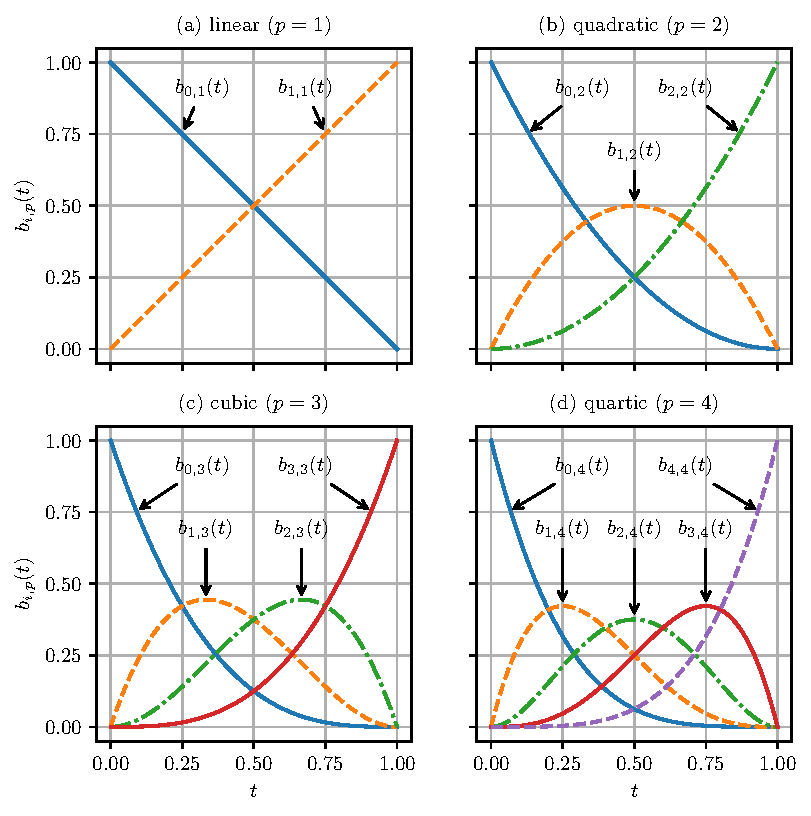
\includegraphics[width=\textwidth]{fig/bernstein.pdf}
  \end{center}
    \caption{Bernstein polynomials for B\'ezier (a) linear, 
    (b) quadratic, 
    (c) cubic, and
    (d) quartic curves.
    Reference: fig/bernstein.py.}
  \label{fig:bernstein} % label must come after caption 
\end{figure}


\clearpage
\section{B\'ezier Surfaces}
The B\'ezier curve was parameterized by $t$.  For the
B\'ezier surface, we have two parameters, $u$ and $v$.
More to come.

